\begin{appendices}
	
	\begin{centerappendixtitle}
		% use centerappendixtitle if the supplementary materials will cover the entire page
		% input the title as usual then insert \pagebreak right after the title
		\chapter{System Flow Chart}
		\pagebreak
		
		\begin{figure}[h]
			\centering
			\caption{Genetic Algorithm}
			\label{genalgoFlow}
			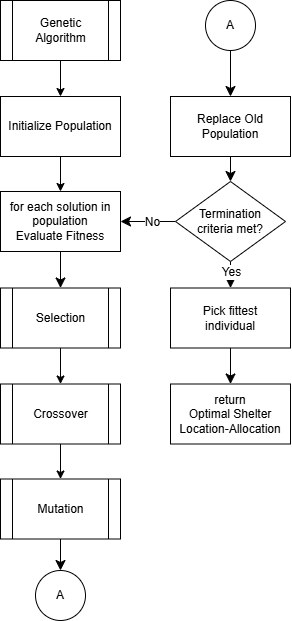
\includegraphics[width=\textwidth,height=\textheight,keepaspectratio]{appendix/Genetic Algorithm Flowchart}
		\end{figure}
		
		\begin{figure}[h]
			\centering
			\caption{Genetic Algorithm - Selection}
			\label{selectFlow}
			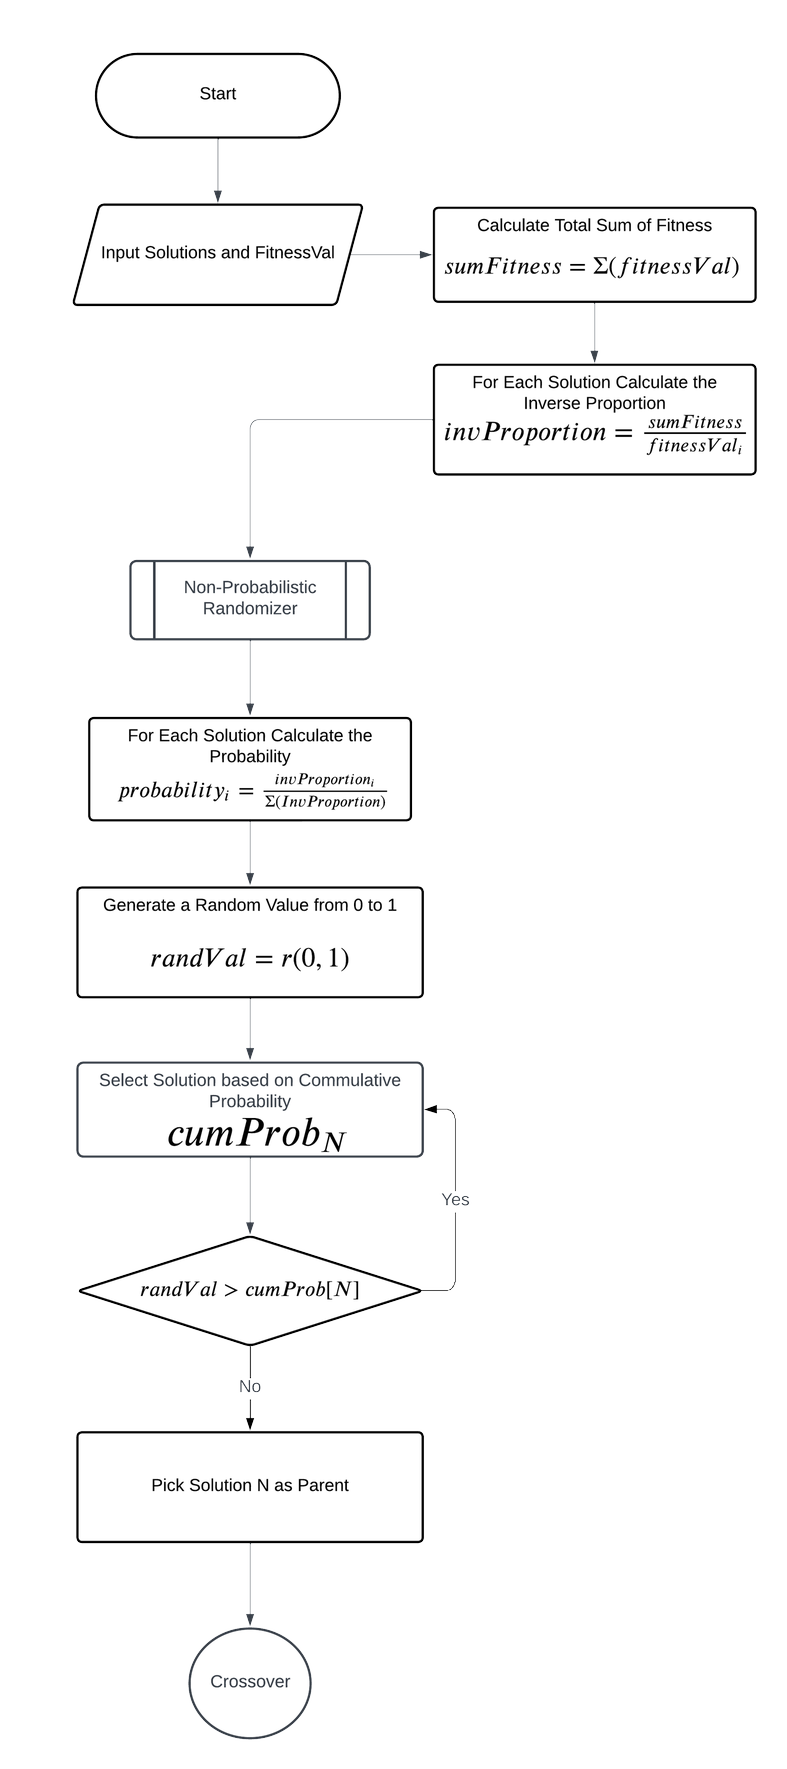
\includegraphics[width=\textwidth,height=\textheight,keepaspectratio]{appendix/select f}
		\end{figure}
		
		\begin{figure}[h]
			\centering
			\caption{Genetic Algorithm - Crossover}
			\label{crossFlow}
			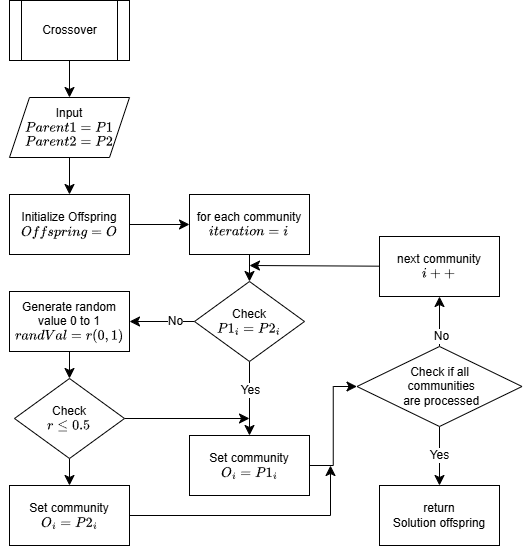
\includegraphics[width=\textwidth,height=\textheight,keepaspectratio]{appendix/crossover f}
		\end{figure}
		
		\begin{figure}[h]
			\centering
			\caption{Genetic Algorithm - Mutation}
			\label{mutateFlow}
			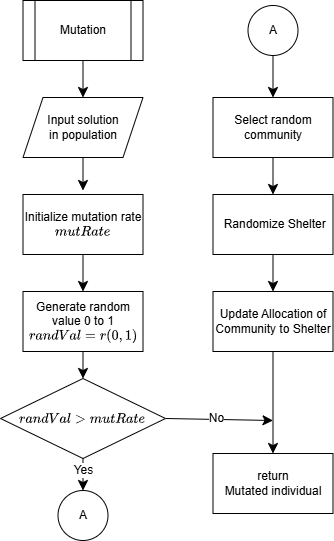
\includegraphics[width=\textwidth,height=\textheight,keepaspectratio]{appendix/mutate f}
		\end{figure}
		
		\begin{figure}[h]
			\centering
			\caption{Data Modification Feature}
			\label{dataModifFlow}
			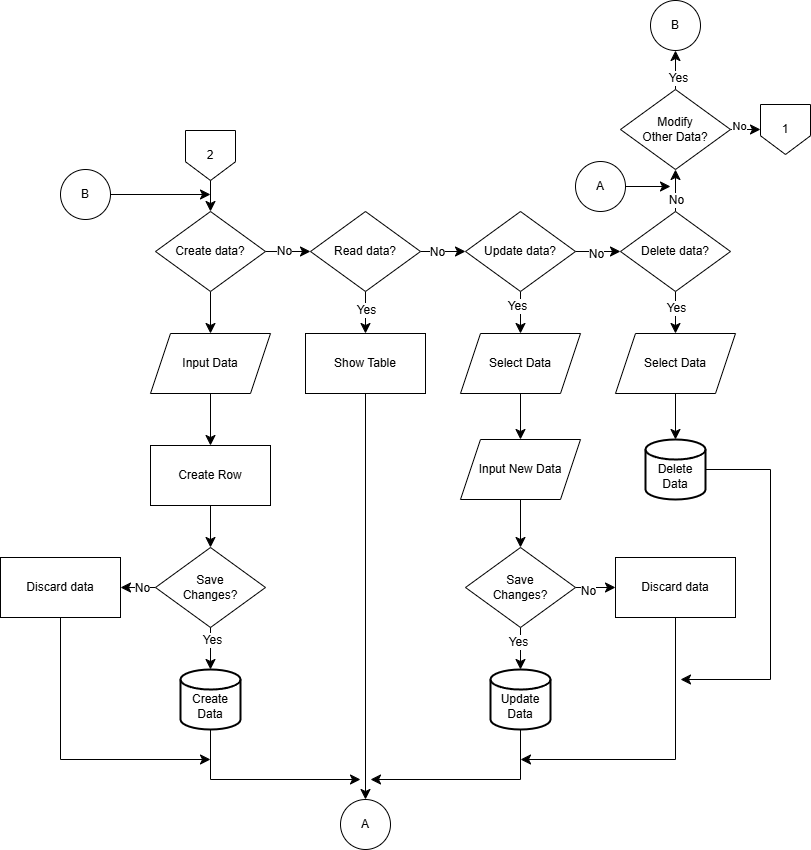
\includegraphics[width=\textwidth,height=\textheight,keepaspectratio]{appendix/data modif f}
		\end{figure}
		
		\begin{figure}[h]
			\centering
			\caption{Model Modification Feature}
			\label{modelFLow}
			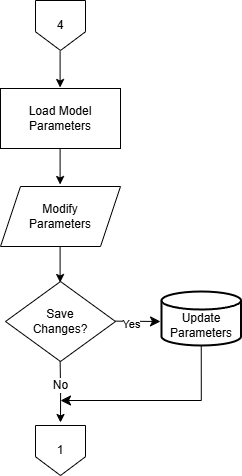
\includegraphics[width=\textwidth,height=\textheight,keepaspectratio]{appendix/modelset f}
		\end{figure}
		
		\begin{figure}[h]
			\centering
			\caption{Data Simulation Feature}
			\label{simFlow}
			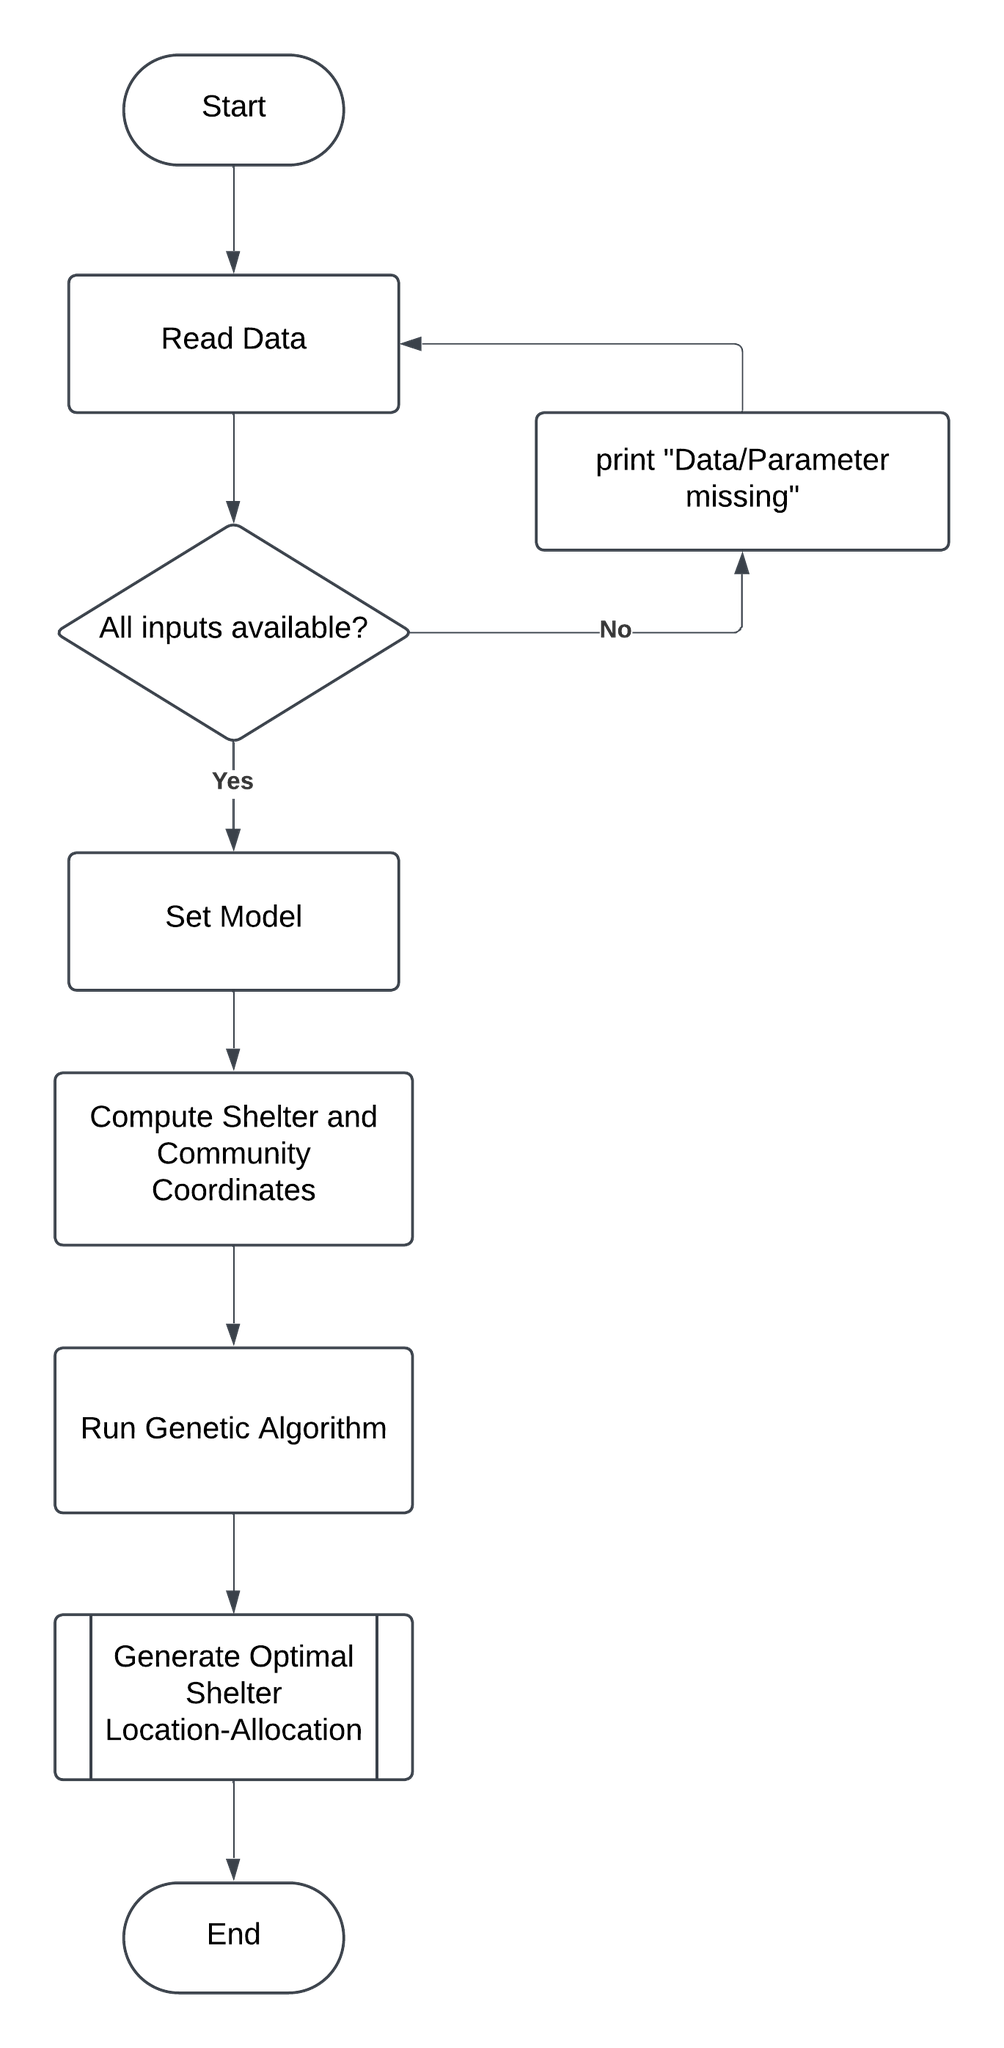
\includegraphics[width=\textwidth,height=\textheight,keepaspectratio]{appendix/datasim f}
		\end{figure}
		
		\begin{figure}[h]
			\centering
			\caption{Shelter Tagging Feature}
			\label{shelTagFlow}
			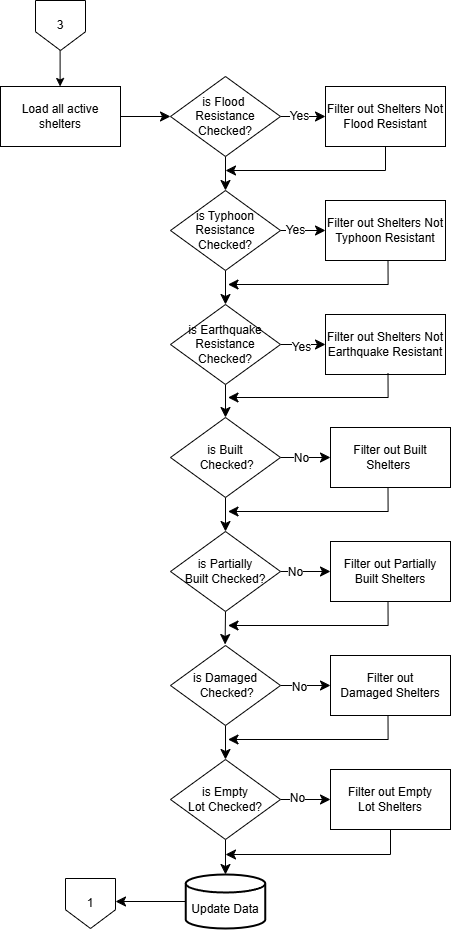
\includegraphics[width=\textwidth,height=\textheight,keepaspectratio]{appendix/sheltertag f}
		\end{figure}
		
		\begin{figure}[h]
			\centering
			\caption{Report Protection Feature}
			\label{protectFlow}
			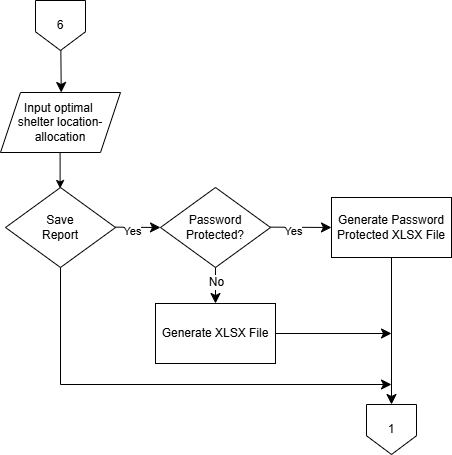
\includegraphics[width=\textwidth,height=\textheight,keepaspectratio]{appendix/protect f}
		\end{figure}
		
		
		
	\end{centerappendixtitle}
	
	\begin{centerappendixtitle}
		% use centerappendixtitle if the supplementary materials will cover the entire page
		% input the title as usual then insert \pagebreak right after the title
		\chapter{Relevant Codes}
		\pagebreak
		
		\begin{figure}[h]
			\centering
			\caption{Genetic Algorithm}
			\label{genalgoCode}
			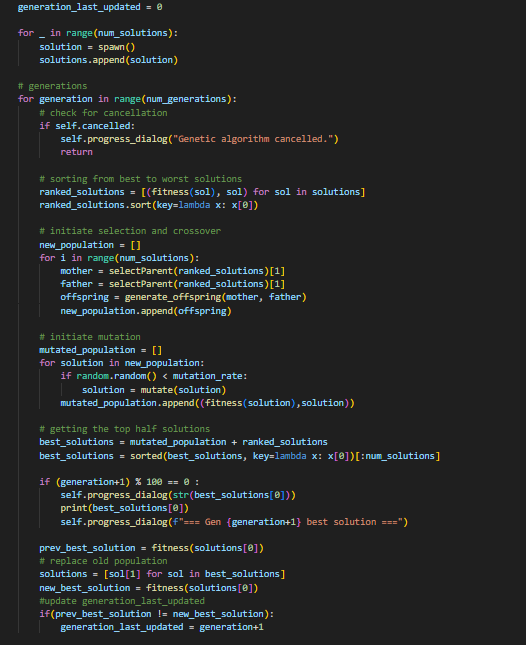
\includegraphics[width=\linewidth]{appendix/gen algo}
		\end{figure}
		
		\begin{figure}[h]
			\centering
			\caption{Genetic Algorithm - Selection}
			\label{selectionCode}
			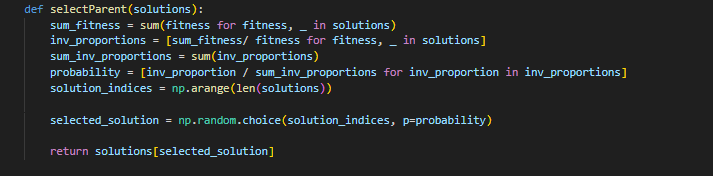
\includegraphics[width=\linewidth]{appendix/selection}
		\end{figure}
		
		\begin{figure}[h]
			\centering
			\caption{Genetic Algorithm - Crossover}
			\label{crossoverCode}
			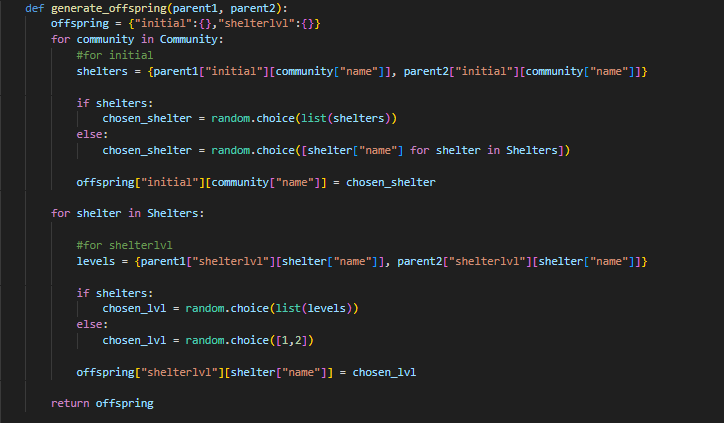
\includegraphics[width=\linewidth]{appendix/crossover}
		\end{figure}
		
		\begin{figure}[h]
			\centering
			\caption{Genetic Algorithm - Mutation}
			\label{mutationCode}
			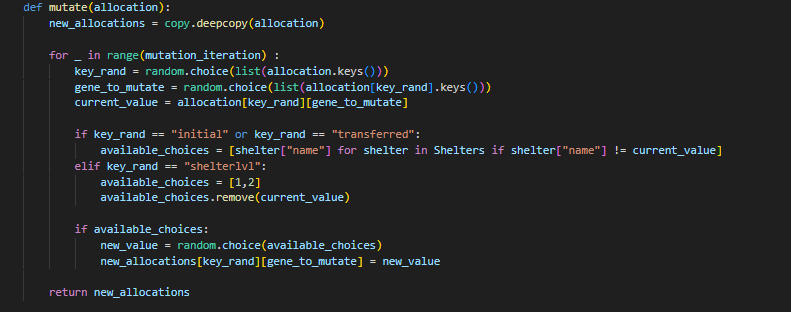
\includegraphics[width=\linewidth]{appendix/mutate}
		\end{figure}
		
		\begin{figure}[h]
			\centering
			\caption{Objective Value}
			\label{objValCode}
			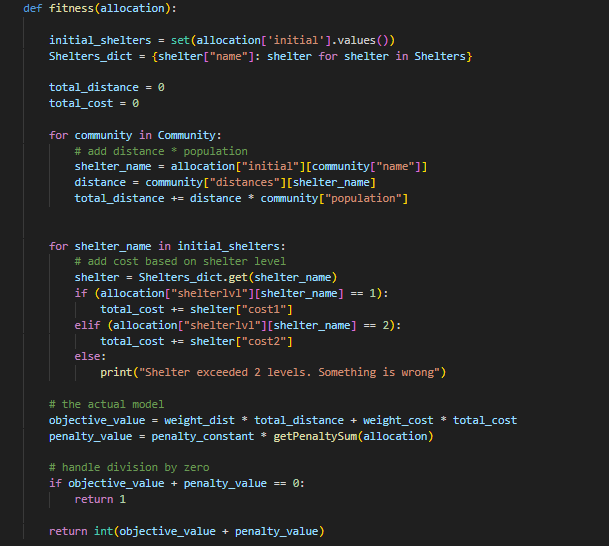
\includegraphics[width=\linewidth]{appendix/fitness}
		\end{figure}
		
		\begin{figure}[h]
			\centering
			\caption{Maximum Distance Constraint}
			\label{maxdistCode}
			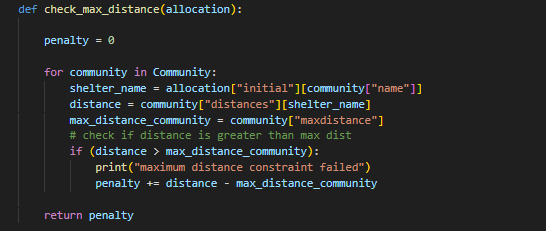
\includegraphics[width=\linewidth]{appendix/dist const}
		\end{figure}
		
		\begin{figure}[h]
			\centering
			\caption{Capacity Constraint}
			\label{capCode}
			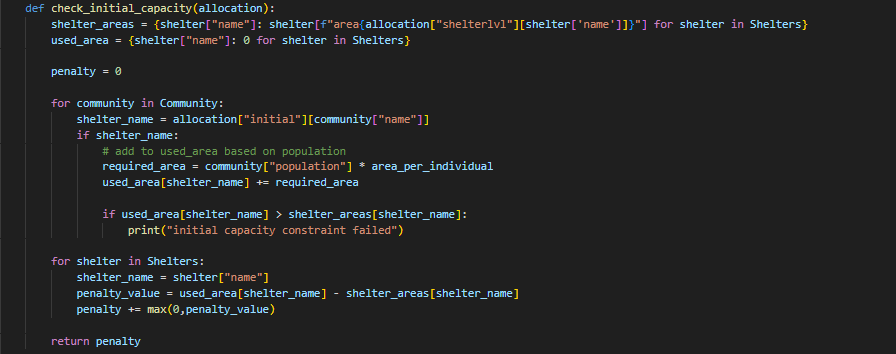
\includegraphics[width=\linewidth]{appendix/capacity const}
		\end{figure}
		
		\begin{figure}[h]
			\centering
			\caption{Maximum Shelter Constraint}
			\label{maxshelCode}
			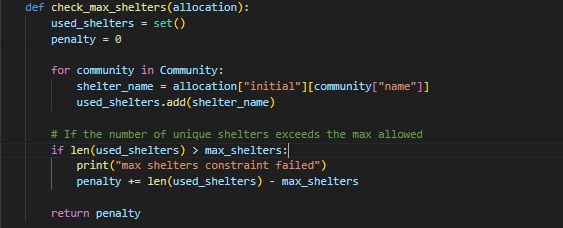
\includegraphics[width=\linewidth]{appendix/max shel const}
		\end{figure}
		
		\begin{figure}[h]
			\centering
			\caption{Maximum Level 2 Shelter Constraint}
			\label{maxl2shelCode}
			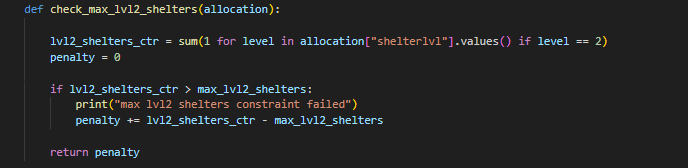
\includegraphics[width=\linewidth]{appendix/max lvl2 shel const}
		\end{figure}
		
		
	\end{centerappendixtitle}
	
	\begin{centerappendixtitle}
		% use centerappendixtitle if the supplementary materials will cover the entire page
		% input the title as usual then insert \pagebreak right after the title
		\chapter{Letters}
		\pagebreak
		
		
\includepdf[pages=1,pagecommand={}]{appendix/Letter-of-Intent-Research-Collab-MDRRMO-Participants}
		
\includepdf[pages=1,pagecommand={}]{appendix/Letter-of-Intent-Research-Collab-MSWDO-Participants}
		\includepdf[pages=-,pagecommand={}]{appendix/Thesis-Endorsement}
		
		
	\end{centerappendixtitle}
	
	\begin{centerappendixtitle}
		% use centerappendixtitle if the supplementary materials will cover the entire page
		% input the title as usual then insert \pagebreak right after the title
		\chapter{Questionnaires}
		\pagebreak
		
		
		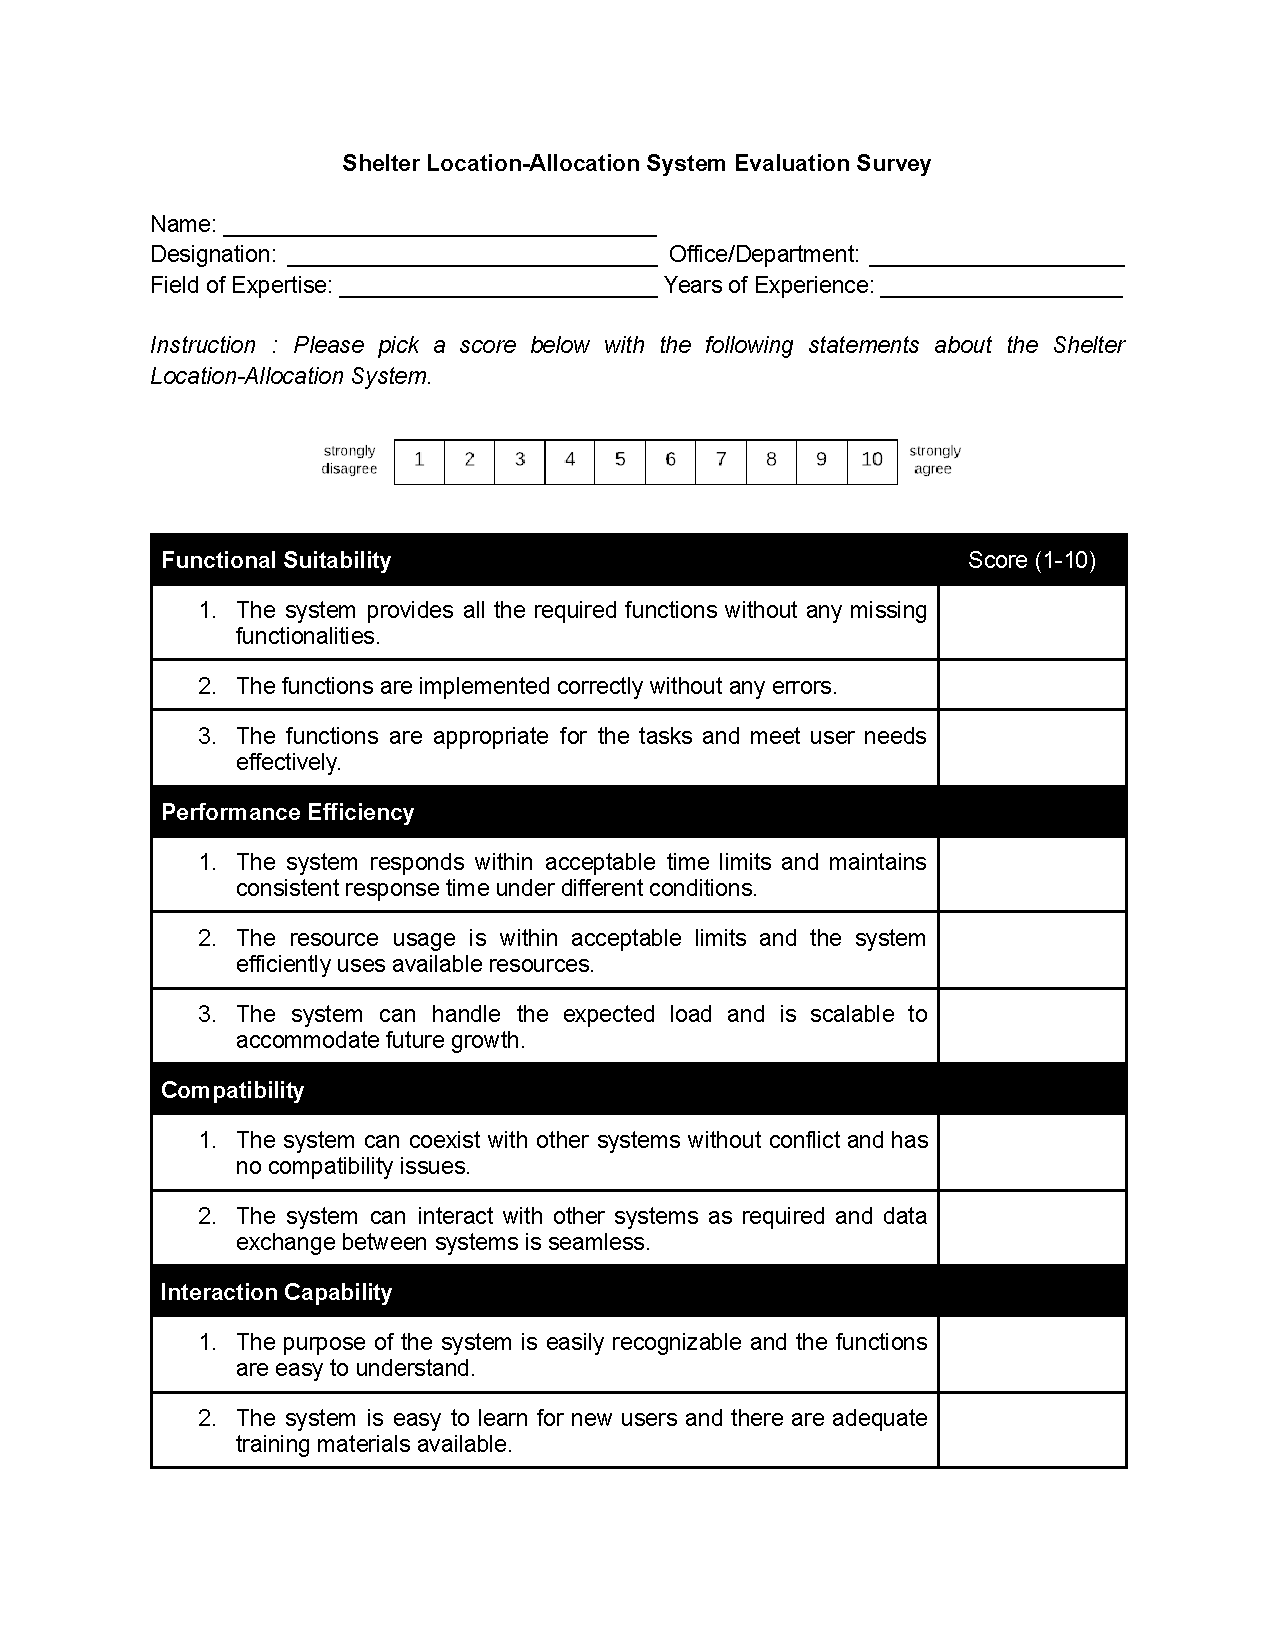
\includepdf[pages=-,pagecommand={}]{appendix/[ISOQuestionnaire]_Thesis}
		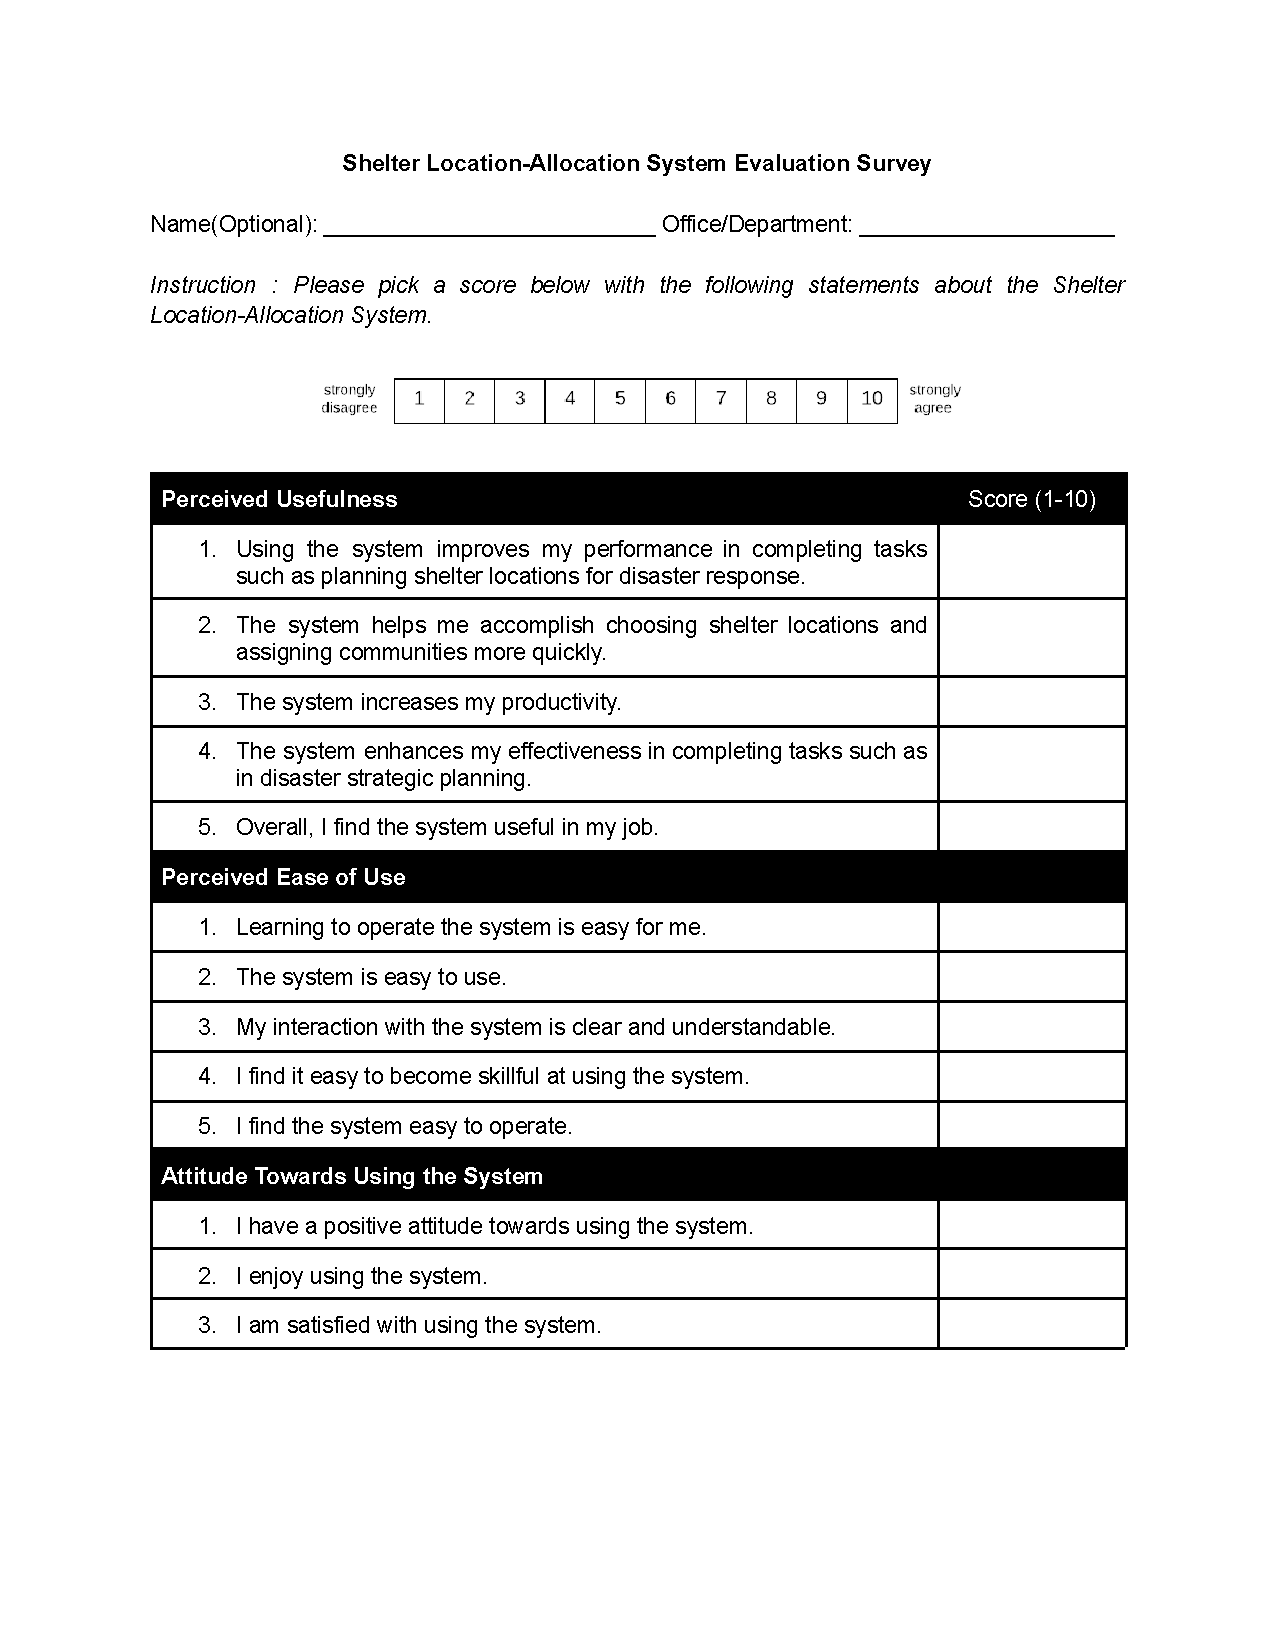
\includepdf[pages=-,pagecommand={}]{appendix/[TAMQuestionnaire]_Thesis}
	\end{centerappendixtitle}
	
	
	
\end{appendices}